\section{MSHR\_\-H Class Reference}
\label{classMSHR__H}\index{MSHR\_\-H@{MSHR\_\-H}}
{\tt \#include $<$mshr.h$>$}

Inheritance diagram for MSHR\_\-H:\nopagebreak
\begin{figure}[H]
\begin{center}
\leavevmode
\includegraphics[height=400pt]{classMSHR__H__inherit__graph}
\end{center}
\end{figure}
Collaboration diagram for MSHR\_\-H:\nopagebreak
\begin{figure}[H]
\begin{center}
\leavevmode
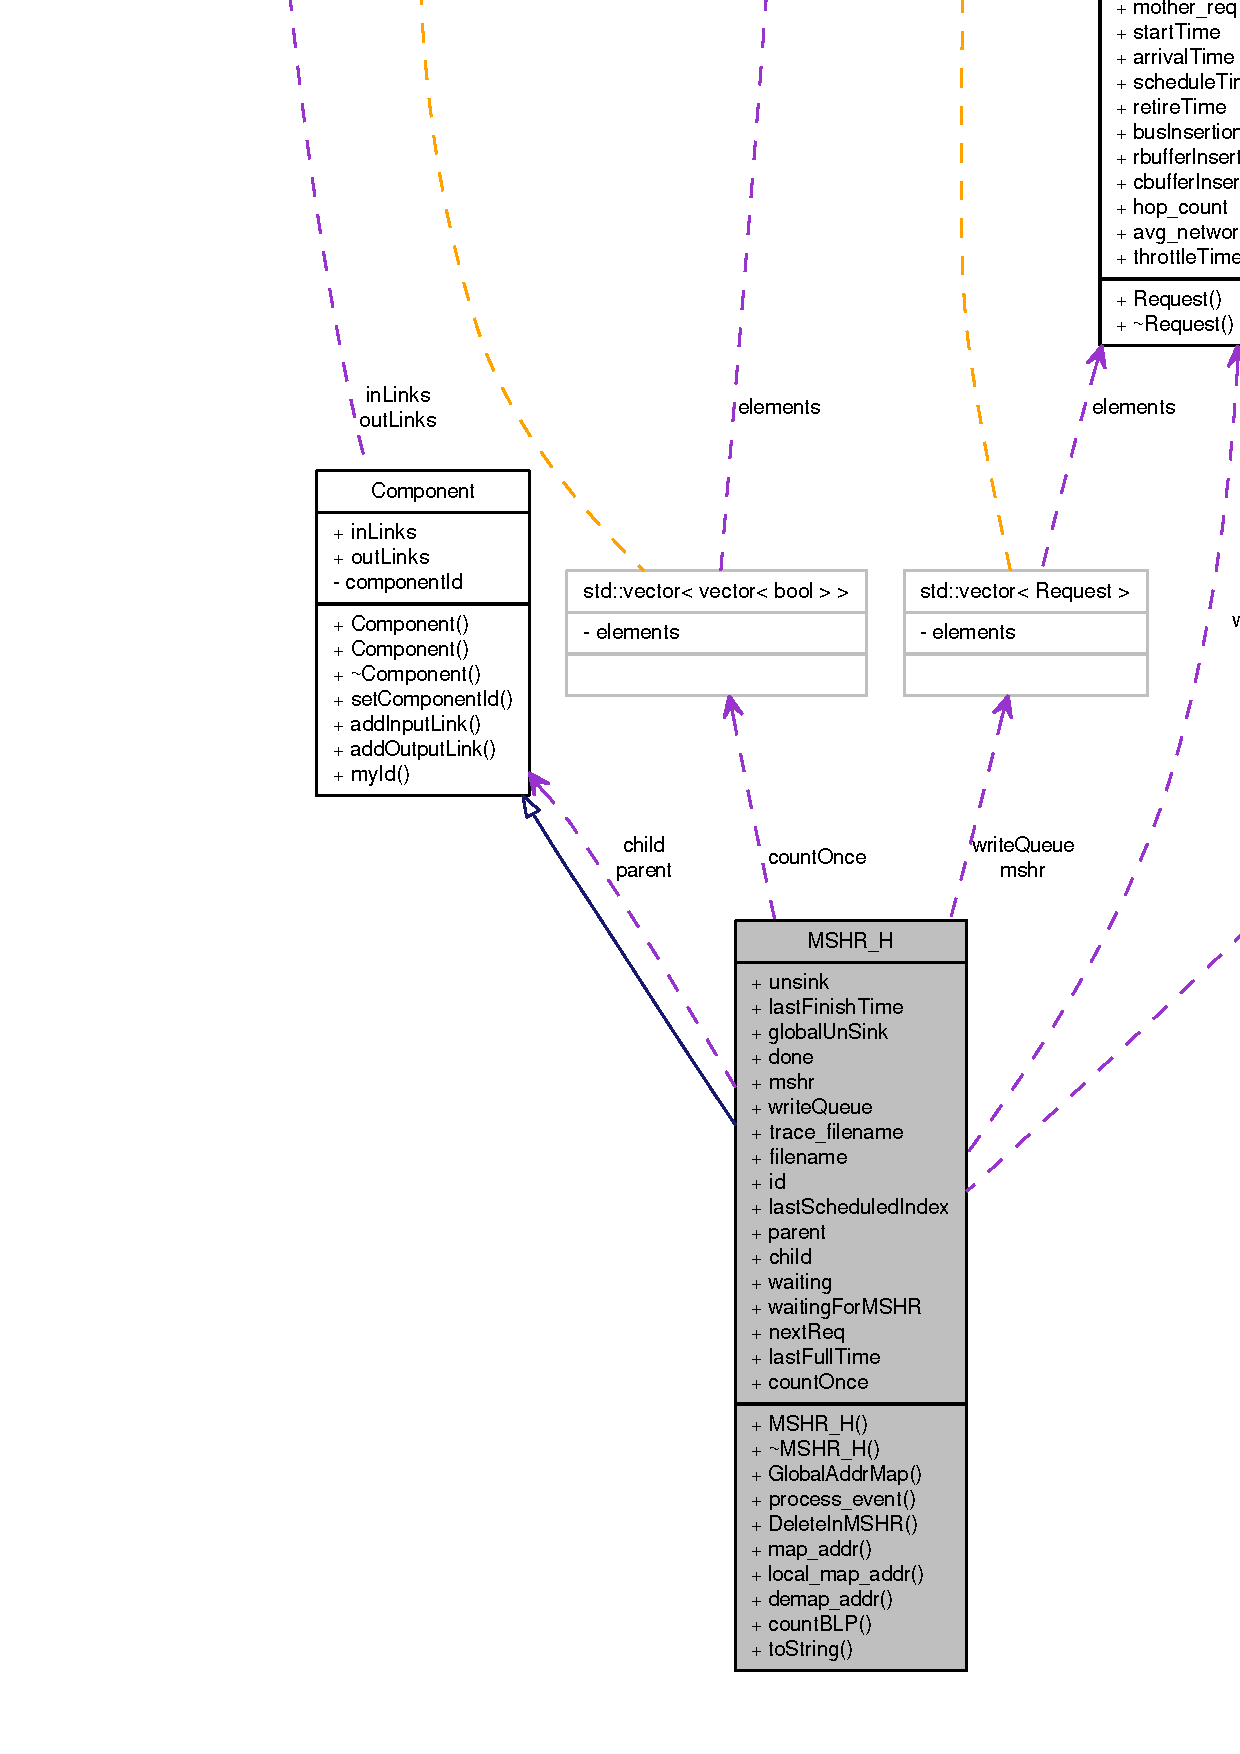
\includegraphics[width=400pt]{classMSHR__H__coll__graph}
\end{center}
\end{figure}
\subsection*{Public Member Functions}
\begin{CompactItemize}
\item 
{\bf MSHR\_\-H} ()
\item 
{\bf $\sim$MSHR\_\-H} ()
\item 
{\bf Addr\_\-t} {\bf GlobalAddrMap} ({\bf Addr\_\-t} addr, {\bf UInt} threadId)
\item 
void {\bf process\_\-event} ({\bf IrisEvent} $\ast$e)
\item 
void {\bf DeleteInMSHR} ({\bf Request} $\ast$req)
\item 
short int {\bf map\_\-addr} (unsigned long long int $\ast$addr)
\item 
void {\bf local\_\-map\_\-addr} ({\bf Request} $\ast$req)
\item 
void {\bf demap\_\-addr} ({\bf Addr\_\-t} oldAddress, {\bf Addr\_\-t} newAddress)
\item 
unsigned int {\bf countBLP} ({\bf Request} req)
\item 
std::string {\bf toString} ()
\end{CompactItemize}
\subsection*{Public Attributes}
\begin{CompactItemize}
\item 
{\bf Time} {\bf unsink}
\item 
{\bf Time} {\bf lastFinishTime}
\item 
{\bf Time} {\bf globalUnSink}
\item 
bool {\bf done}
\item 
vector$<$ {\bf Request} $>$ {\bf mshr}
\item 
vector$<$ {\bf Request} $>$ {\bf writeQueue}
\item 
ifstream {\bf trace\_\-filename}
\item 
char $\ast$ {\bf filename}
\item 
unsigned int {\bf id}
\item 
unsigned int {\bf lastScheduledIndex}
\item 
{\bf Component} $\ast$ {\bf parent}
\item 
{\bf Component} $\ast$ {\bf child}
\item 
bool {\bf waiting}
\item 
{\bf Request} {\bf waitingForMSHR}
\item 
{\bf Request} {\bf nextReq}
\item 
{\bf Time} {\bf lastFullTime}
\item 
vector$<$ vector$<$ bool $>$ $>$ {\bf countOnce}
\end{CompactItemize}


\subsection{Detailed Description}


Definition at line 50 of file mshr.h.

\subsection{Constructor \& Destructor Documentation}
\index{MSHR\_\-H@{MSHR\_\-H}!MSHR\_\-H@{MSHR\_\-H}}
\index{MSHR\_\-H@{MSHR\_\-H}!MSHR_H@{MSHR\_\-H}}
\subsubsection[{MSHR\_\-H}]{\setlength{\rightskip}{0pt plus 5cm}MSHR\_\-H::MSHR\_\-H ()}\label{classMSHR__H_ed75aac9537ffb4d5814b337c1099e82}




Definition at line 36 of file mshr.cc.

References countOnce, done, globalUnSink, lastFinishTime, lastFullTime, lastScheduledIndex, mshr, no\_\-mcs, NO\_\-OF\_\-BANKS, unsink, waiting, and writeQueue.\index{MSHR\_\-H@{MSHR\_\-H}!$\sim$MSHR\_\-H@{$\sim$MSHR\_\-H}}
\index{$\sim$MSHR\_\-H@{$\sim$MSHR\_\-H}!MSHR_H@{MSHR\_\-H}}
\subsubsection[{$\sim$MSHR\_\-H}]{\setlength{\rightskip}{0pt plus 5cm}MSHR\_\-H::$\sim$MSHR\_\-H ()}\label{classMSHR__H_cbe3ee20d72b496c43ef9f6375f4da1b}




Definition at line 59 of file mshr.cc.

References mshr, and writeQueue.

\subsection{Member Function Documentation}
\index{MSHR\_\-H@{MSHR\_\-H}!countBLP@{countBLP}}
\index{countBLP@{countBLP}!MSHR_H@{MSHR\_\-H}}
\subsubsection[{countBLP}]{\setlength{\rightskip}{0pt plus 5cm}unsigned int MSHR\_\-H::countBLP ({\bf Request} {\em req})}\label{classMSHR__H_5da0445647a27cbacf66210de6f88f71}




Definition at line 262 of file mshr.cc.

References countOnce, lastScheduledIndex, mshr, no\_\-mcs, and NO\_\-OF\_\-BANKS.\index{MSHR\_\-H@{MSHR\_\-H}!DeleteInMSHR@{DeleteInMSHR}}
\index{DeleteInMSHR@{DeleteInMSHR}!MSHR_H@{MSHR\_\-H}}
\subsubsection[{DeleteInMSHR}]{\setlength{\rightskip}{0pt plus 5cm}void MSHR\_\-H::DeleteInMSHR ({\bf Request} $\ast$ {\em req})}\label{classMSHR__H_11c3517e46d1f3dfc36ab540939ae3dd}




Definition at line 240 of file mshr.cc.

References Request::address, lastScheduledIndex, Request::mcNo, mshr, Simulator::Now(), parent, and Request::startTime.

Referenced by process\_\-event().

Here is the caller graph for this function:\nopagebreak
\begin{figure}[H]
\begin{center}
\leavevmode
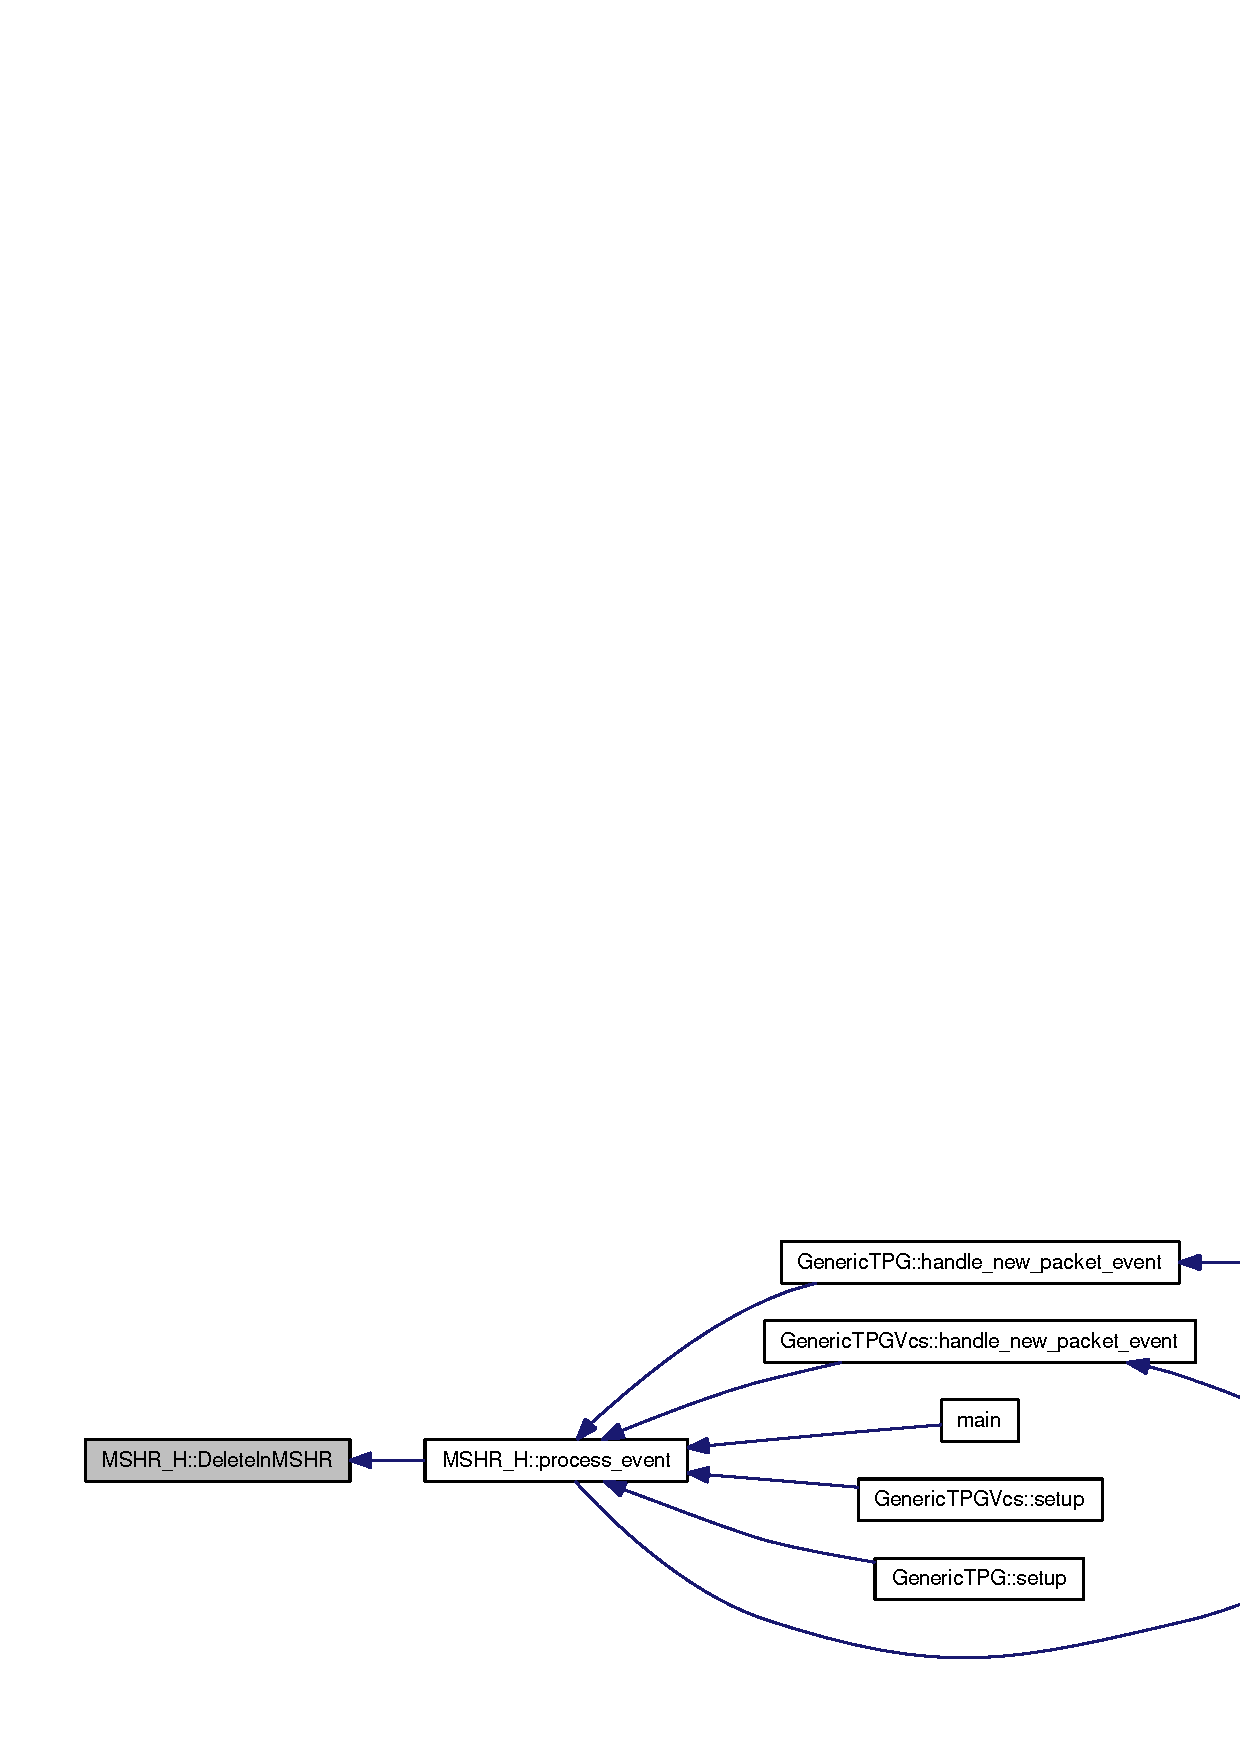
\includegraphics[width=385pt]{classMSHR__H_11c3517e46d1f3dfc36ab540939ae3dd_icgraph}
\end{center}
\end{figure}
\index{MSHR\_\-H@{MSHR\_\-H}!demap\_\-addr@{demap\_\-addr}}
\index{demap\_\-addr@{demap\_\-addr}!MSHR_H@{MSHR\_\-H}}
\subsubsection[{demap\_\-addr}]{\setlength{\rightskip}{0pt plus 5cm}void MSHR\_\-H::demap\_\-addr ({\bf Addr\_\-t} {\em oldAddress}, \/  {\bf Addr\_\-t} {\em newAddress})}\label{classMSHR__H_d0214a2b87adc1e701052c2f4abe759f}




Definition at line 285 of file mshr.cc.

References mshr, and Simulator::Now().\index{MSHR\_\-H@{MSHR\_\-H}!GlobalAddrMap@{GlobalAddrMap}}
\index{GlobalAddrMap@{GlobalAddrMap}!MSHR_H@{MSHR\_\-H}}
\subsubsection[{GlobalAddrMap}]{\setlength{\rightskip}{0pt plus 5cm}{\bf Addr\_\-t} MSHR\_\-H::GlobalAddrMap ({\bf Addr\_\-t} {\em addr}, \/  {\bf UInt} {\em threadId})}\label{classMSHR__H_3c9cdbe3938dcfd521f48678b335b839}




Definition at line 225 of file mshr.cc.

References NO\_\-OF\_\-THREADS, and THREAD\_\-BITS\_\-POSITION.

Referenced by GenericTPGVcs::GetNextRequest(), GenericTPG::GetNextRequest(), main(), process\_\-event(), GenericTPGVcs::setup(), and GenericTPG::setup().

Here is the caller graph for this function:\nopagebreak
\begin{figure}[H]
\begin{center}
\leavevmode
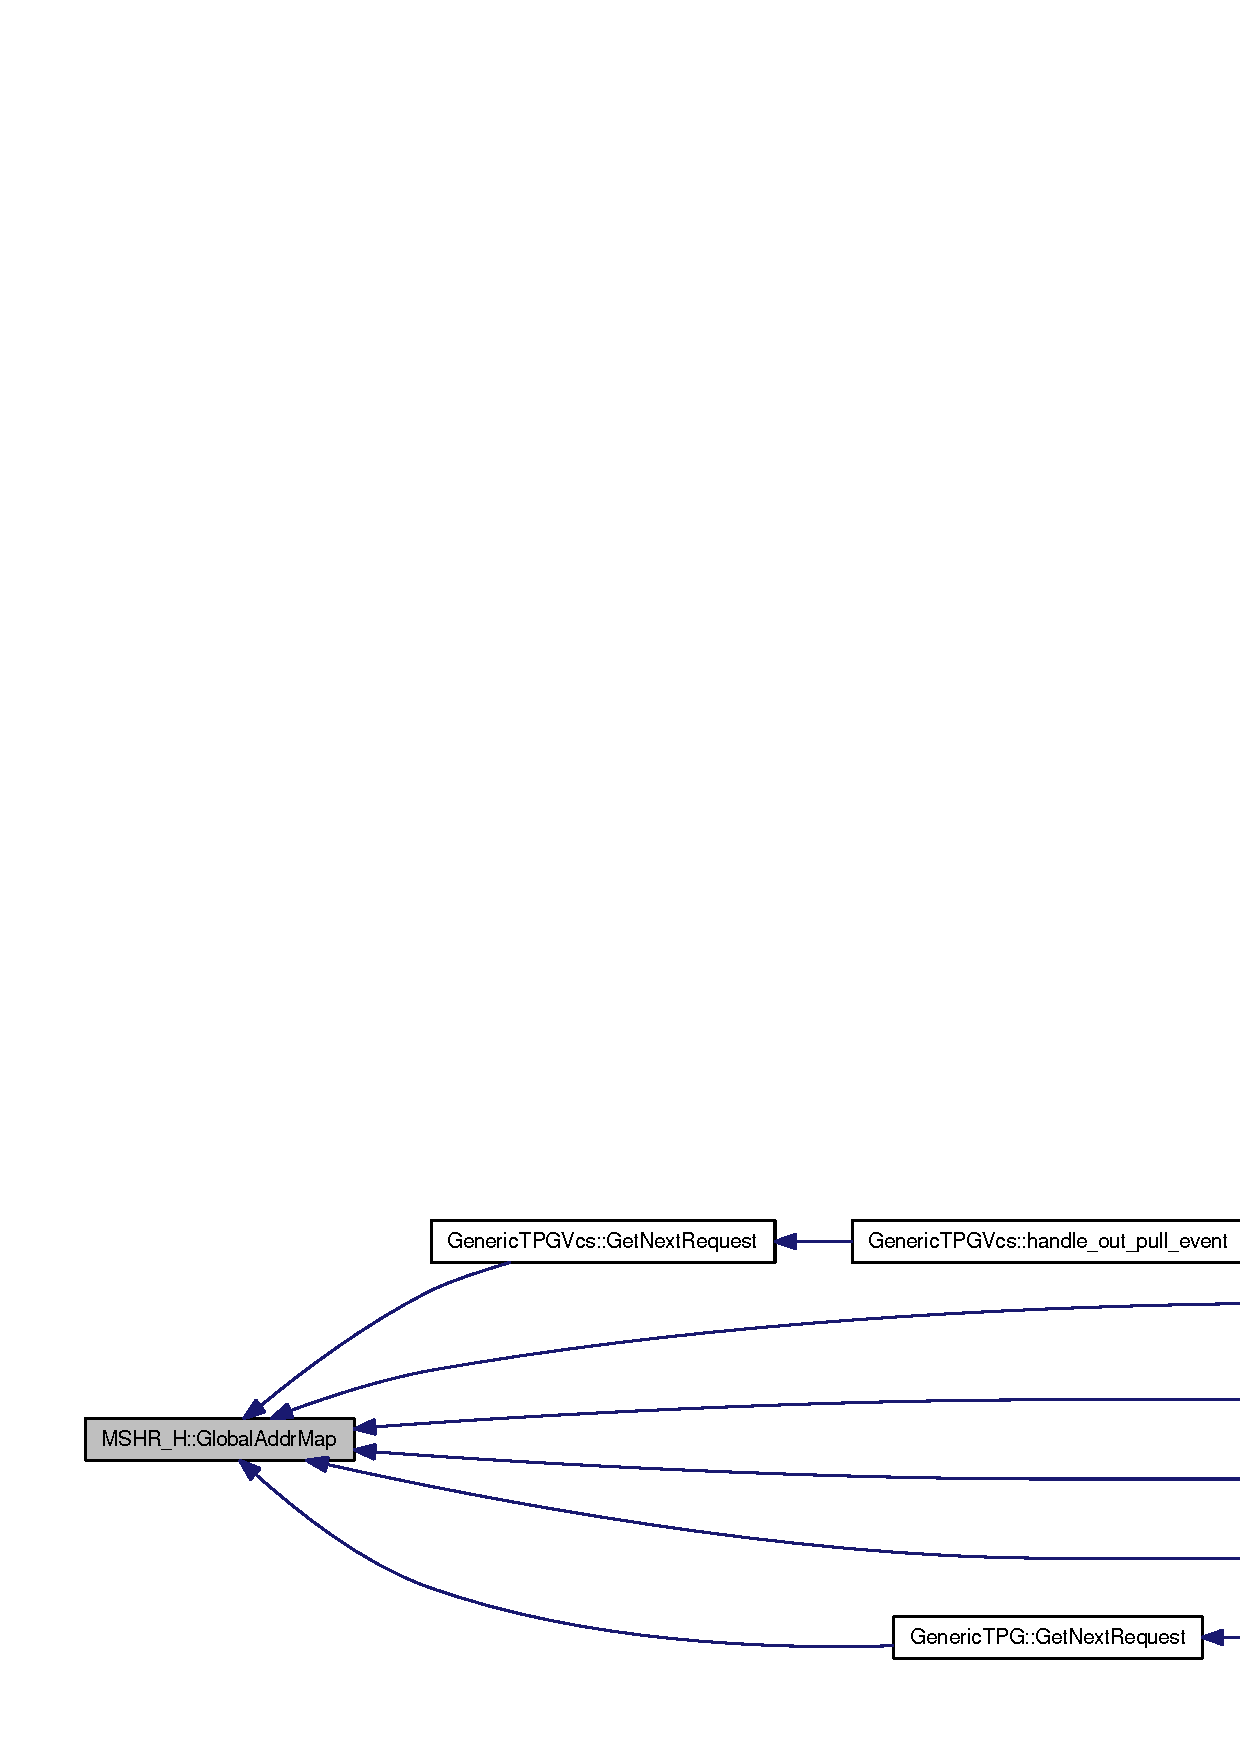
\includegraphics[width=420pt]{classMSHR__H_3c9cdbe3938dcfd521f48678b335b839_icgraph}
\end{center}
\end{figure}
\index{MSHR\_\-H@{MSHR\_\-H}!local\_\-map\_\-addr@{local\_\-map\_\-addr}}
\index{local\_\-map\_\-addr@{local\_\-map\_\-addr}!MSHR_H@{MSHR\_\-H}}
\subsubsection[{local\_\-map\_\-addr}]{\setlength{\rightskip}{0pt plus 5cm}void MSHR\_\-H::local\_\-map\_\-addr ({\bf Request} $\ast$ {\em req})}\label{classMSHR__H_31a63345b220f9e3eaefc9b4eb012f6b}




Definition at line 325 of file mshr.cc.

References Request::address, Request::bankNo, BLOCKS\_\-PER\_\-ROW, CACHE\_\-BLOCK\_\-SIZE, Request::channelNo, COLUMN\_\-SIZE, Request::columnNo, DRAM\_\-SIZE, Request::lowerBits, NO\_\-OF\_\-BANKS, NO\_\-OF\_\-CHANNELS, NO\_\-OF\_\-COLUMNS, NO\_\-OF\_\-RANKS, NO\_\-OF\_\-ROWS, Request::rankNo, ROW\_\-SIZE, Request::rowNo, and TAG\_\-BITS.

Referenced by process\_\-event().

Here is the caller graph for this function:\nopagebreak
\begin{figure}[H]
\begin{center}
\leavevmode
\includegraphics[width=387pt]{classMSHR__H_31a63345b220f9e3eaefc9b4eb012f6b_icgraph}
\end{center}
\end{figure}
\index{MSHR\_\-H@{MSHR\_\-H}!map\_\-addr@{map\_\-addr}}
\index{map\_\-addr@{map\_\-addr}!MSHR_H@{MSHR\_\-H}}
\subsubsection[{map\_\-addr}]{\setlength{\rightskip}{0pt plus 5cm}short int MSHR\_\-H::map\_\-addr (unsigned long long int $\ast$ {\em addr})}\label{classMSHR__H_aeb79565c3b2b9058ae8e270f739ae6d}




Definition at line 304 of file mshr.cc.

References MC\_\-ADDR\_\-BITS, no\_\-mcs, and NO\_\-OF\_\-THREADS.

Referenced by process\_\-event().

Here is the caller graph for this function:\nopagebreak
\begin{figure}[H]
\begin{center}
\leavevmode
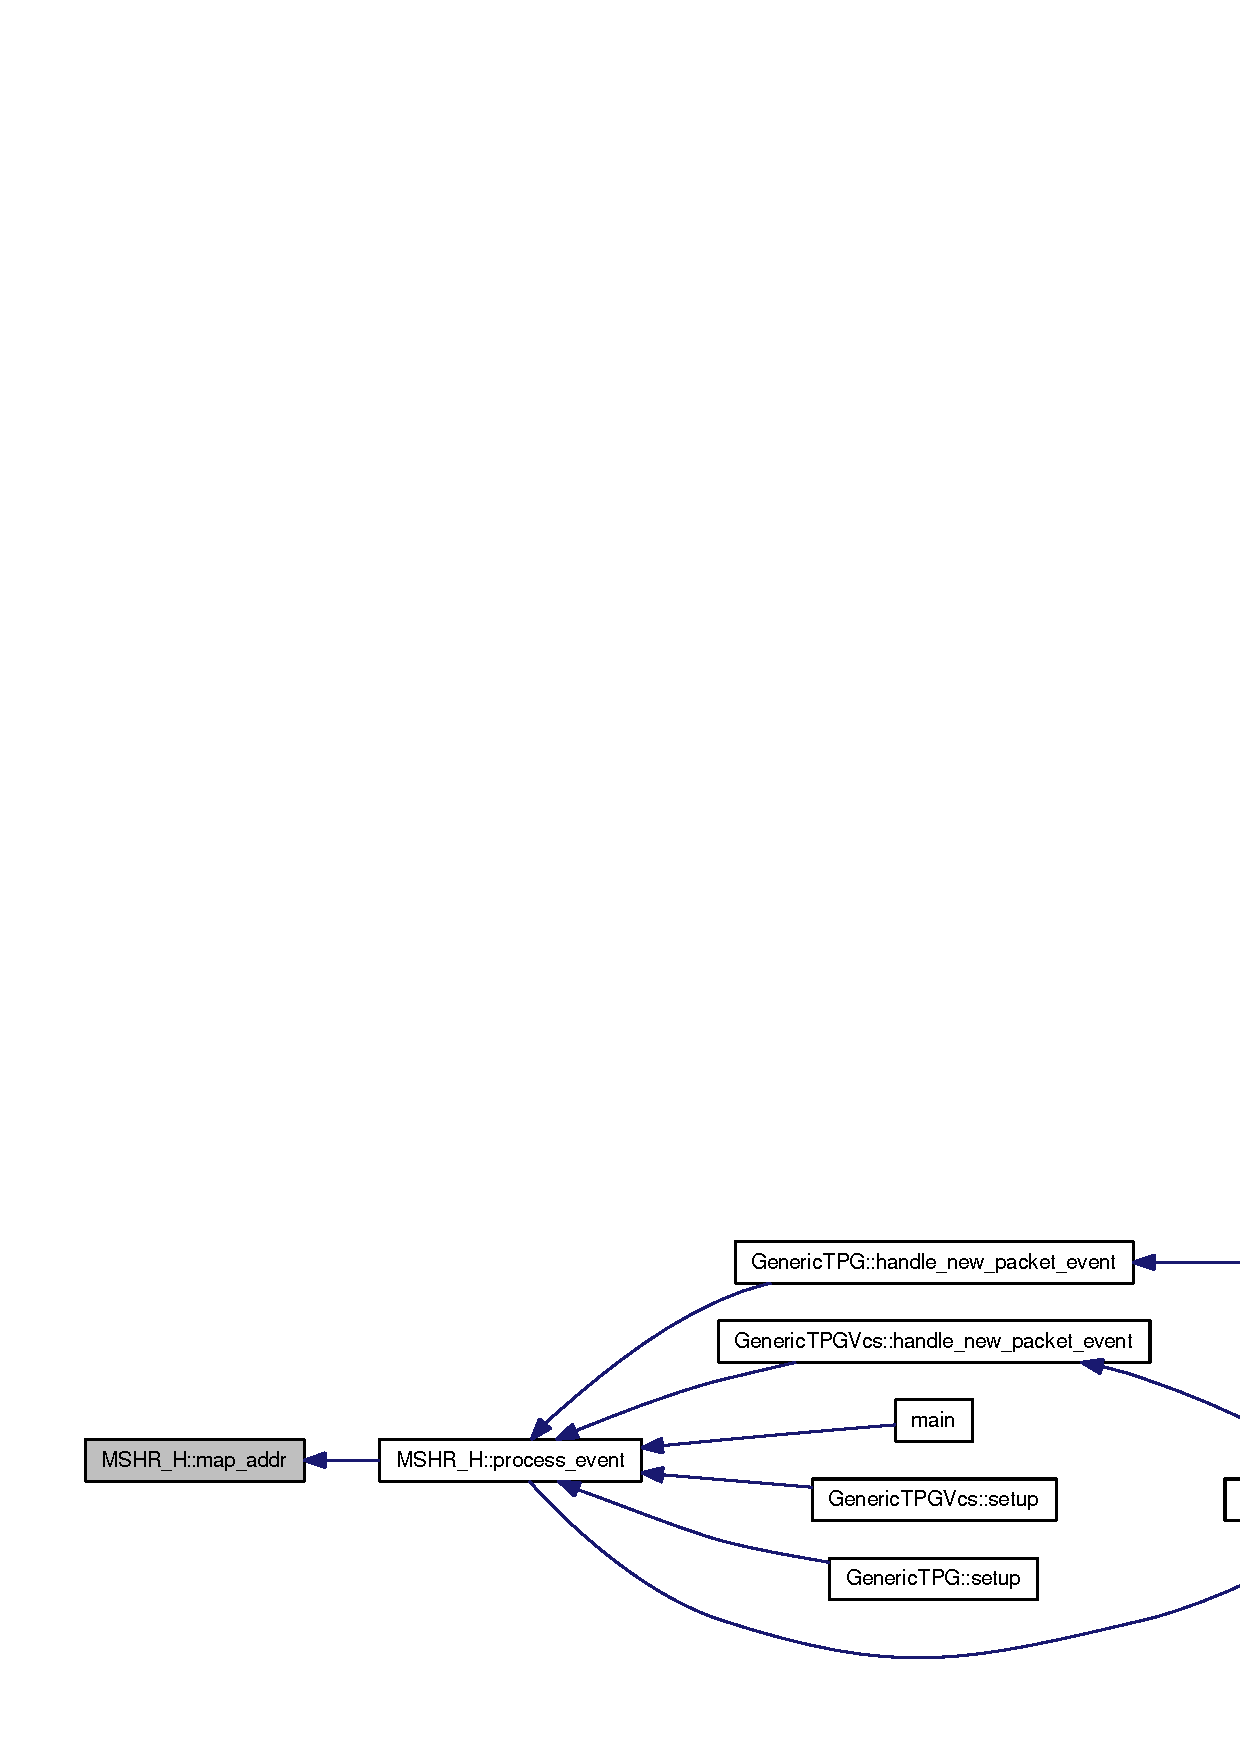
\includegraphics[width=374pt]{classMSHR__H_aeb79565c3b2b9058ae8e270f739ae6d_icgraph}
\end{center}
\end{figure}
\index{MSHR\_\-H@{MSHR\_\-H}!process\_\-event@{process\_\-event}}
\index{process\_\-event@{process\_\-event}!MSHR_H@{MSHR\_\-H}}
\subsubsection[{process\_\-event}]{\setlength{\rightskip}{0pt plus 5cm}void MSHR\_\-H::process\_\-event ({\bf IrisEvent} $\ast$ {\em e})}\label{classMSHR__H_1dff946e7d92eae286b8f72df7dc0f03}




Definition at line 72 of file mshr.cc.

References Request::address, Request::arrivalTime, CACHE\_\-WRITEBACK, Request::cmdType, DeleteInMSHR(), done, IrisEvent::dst, IrisEvent::event\_\-data, filename, GlobalAddrMap(), globalUnSink, id, lastFinishTime, lastFullTime, local\_\-map\_\-addr(), map\_\-addr(), max\_\-sim\_\-time, Request::mcNo, mshr, MSHR\_\-DELETE, MSHR\_\-SIZE, nextReq, Simulator::Now(), OUT\_\-PULL\_\-EVENT, parent, GenericTPGVcs::process\_\-event(), Simulator::Schedule(), IrisEvent::src, Request::startTime, Request::threadId, trace\_\-filename, IrisEvent::type, unsink, waiting, waitingForMSHR, and writeQueue.

Referenced by GenericTPGVcs::handle\_\-new\_\-packet\_\-event(), GenericTPG::handle\_\-new\_\-packet\_\-event(), main(), GenericTPGVcs::setup(), and GenericTPG::setup().

Here is the caller graph for this function:\nopagebreak
\begin{figure}[H]
\begin{center}
\leavevmode
\includegraphics[width=303pt]{classMSHR__H_1dff946e7d92eae286b8f72df7dc0f03_icgraph}
\end{center}
\end{figure}
\index{MSHR\_\-H@{MSHR\_\-H}!toString@{toString}}
\index{toString@{toString}!MSHR_H@{MSHR\_\-H}}
\subsubsection[{toString}]{\setlength{\rightskip}{0pt plus 5cm}std::string MSHR\_\-H::toString ()}\label{classMSHR__H_778e0a25bf58c2ccbe506a4c635f953f}




\subsection{Member Data Documentation}
\index{MSHR\_\-H@{MSHR\_\-H}!child@{child}}
\index{child@{child}!MSHR_H@{MSHR\_\-H}}
\subsubsection[{child}]{\setlength{\rightskip}{0pt plus 5cm}{\bf Component}$\ast$ {\bf MSHR\_\-H::child}}\label{classMSHR__H_4806bb8e724a54f993b119bd9b4542fd}




Definition at line 66 of file mshr.h.\index{MSHR\_\-H@{MSHR\_\-H}!countOnce@{countOnce}}
\index{countOnce@{countOnce}!MSHR_H@{MSHR\_\-H}}
\subsubsection[{countOnce}]{\setlength{\rightskip}{0pt plus 5cm}vector$<$ vector$<$bool$>$ $>$ {\bf MSHR\_\-H::countOnce}}\label{classMSHR__H_788db7ac4c7430daf82deb2fd21f3316}




Definition at line 79 of file mshr.h.

Referenced by countBLP(), and MSHR\_\-H().\index{MSHR\_\-H@{MSHR\_\-H}!done@{done}}
\index{done@{done}!MSHR_H@{MSHR\_\-H}}
\subsubsection[{done}]{\setlength{\rightskip}{0pt plus 5cm}bool {\bf MSHR\_\-H::done}}\label{classMSHR__H_4cd1713ebd3ab9038ed231781b4bc36a}




Definition at line 58 of file mshr.h.

Referenced by main(), MSHR\_\-H(), and process\_\-event().\index{MSHR\_\-H@{MSHR\_\-H}!filename@{filename}}
\index{filename@{filename}!MSHR_H@{MSHR\_\-H}}
\subsubsection[{filename}]{\setlength{\rightskip}{0pt plus 5cm}char$\ast$ {\bf MSHR\_\-H::filename}}\label{classMSHR__H_2625121a72d102823d11503459b6322c}




Definition at line 62 of file mshr.h.

Referenced by main(), process\_\-event(), GenericTPGVcs::setup(), and GenericTPG::setup().\index{MSHR\_\-H@{MSHR\_\-H}!globalUnSink@{globalUnSink}}
\index{globalUnSink@{globalUnSink}!MSHR_H@{MSHR\_\-H}}
\subsubsection[{globalUnSink}]{\setlength{\rightskip}{0pt plus 5cm}{\bf Time} {\bf MSHR\_\-H::globalUnSink}}\label{classMSHR__H_08f7e602a70bcf8d0e991d46e19265a2}




Definition at line 57 of file mshr.h.

Referenced by main(), MSHR\_\-H(), and process\_\-event().\index{MSHR\_\-H@{MSHR\_\-H}!id@{id}}
\index{id@{id}!MSHR_H@{MSHR\_\-H}}
\subsubsection[{id}]{\setlength{\rightskip}{0pt plus 5cm}unsigned int {\bf MSHR\_\-H::id}}\label{classMSHR__H_97b745c7aeca64268c19411dd6ba5354}




Definition at line 63 of file mshr.h.

Referenced by main(), process\_\-event(), GenericTPGVcs::setup(), and GenericTPG::setup().\index{MSHR\_\-H@{MSHR\_\-H}!lastFinishTime@{lastFinishTime}}
\index{lastFinishTime@{lastFinishTime}!MSHR_H@{MSHR\_\-H}}
\subsubsection[{lastFinishTime}]{\setlength{\rightskip}{0pt plus 5cm}{\bf Time} {\bf MSHR\_\-H::lastFinishTime}}\label{classMSHR__H_adfd06c0a14ec47c72e3b3e0c436d62e}




Definition at line 56 of file mshr.h.

Referenced by MSHR\_\-H(), and process\_\-event().\index{MSHR\_\-H@{MSHR\_\-H}!lastFullTime@{lastFullTime}}
\index{lastFullTime@{lastFullTime}!MSHR_H@{MSHR\_\-H}}
\subsubsection[{lastFullTime}]{\setlength{\rightskip}{0pt plus 5cm}{\bf Time} {\bf MSHR\_\-H::lastFullTime}}\label{classMSHR__H_d00d664b7b00f6778cb5ec4ed33b8ca6}




Definition at line 77 of file mshr.h.

Referenced by MSHR\_\-H(), and process\_\-event().\index{MSHR\_\-H@{MSHR\_\-H}!lastScheduledIndex@{lastScheduledIndex}}
\index{lastScheduledIndex@{lastScheduledIndex}!MSHR_H@{MSHR\_\-H}}
\subsubsection[{lastScheduledIndex}]{\setlength{\rightskip}{0pt plus 5cm}unsigned int {\bf MSHR\_\-H::lastScheduledIndex}}\label{classMSHR__H_fd269df00bf476b2b151516b64cf7388}




Definition at line 64 of file mshr.h.

Referenced by countBLP(), DeleteInMSHR(), GenericTPGVcs::GetNewRequest(), GenericTPG::GetNewRequest(), GetNextRequest(), GenericTPG::handle\_\-out\_\-pull\_\-event(), and MSHR\_\-H().\index{MSHR\_\-H@{MSHR\_\-H}!mshr@{mshr}}
\index{mshr@{mshr}!MSHR_H@{MSHR\_\-H}}
\subsubsection[{mshr}]{\setlength{\rightskip}{0pt plus 5cm}vector$<${\bf Request}$>$ {\bf MSHR\_\-H::mshr}}\label{classMSHR__H_993765f65d7a1b94d3340bc166aab1f4}




Definition at line 59 of file mshr.h.

Referenced by countBLP(), DeleteInMSHR(), demap\_\-addr(), GenericTPGVcs::GetNewRequest(), GenericTPG::GetNewRequest(), GetNextRequest(), GenericTPGVcs::handle\_\-out\_\-pull\_\-event(), GenericTPG::handle\_\-out\_\-pull\_\-event(), MSHR\_\-H(), process\_\-event(), GenericTPG::$\sim$GenericTPG(), GenericTPGVcs::$\sim$GenericTPGVcs(), and $\sim$MSHR\_\-H().\index{MSHR\_\-H@{MSHR\_\-H}!nextReq@{nextReq}}
\index{nextReq@{nextReq}!MSHR_H@{MSHR\_\-H}}
\subsubsection[{nextReq}]{\setlength{\rightskip}{0pt plus 5cm}{\bf Request} {\bf MSHR\_\-H::nextReq}}\label{classMSHR__H_e27c92520271fd9c341f705c1d8d6a50}




Definition at line 76 of file mshr.h.

Referenced by process\_\-event().\index{MSHR\_\-H@{MSHR\_\-H}!parent@{parent}}
\index{parent@{parent}!MSHR_H@{MSHR\_\-H}}
\subsubsection[{parent}]{\setlength{\rightskip}{0pt plus 5cm}{\bf Component}$\ast$ {\bf MSHR\_\-H::parent}}\label{classMSHR__H_d230dd4ae492389c1b03255bb76261fa}




Definition at line 65 of file mshr.h.

Referenced by DeleteInMSHR(), process\_\-event(), GenericTPGVcs::setup(), and GenericTPG::setup().\index{MSHR\_\-H@{MSHR\_\-H}!trace\_\-filename@{trace\_\-filename}}
\index{trace\_\-filename@{trace\_\-filename}!MSHR_H@{MSHR\_\-H}}
\subsubsection[{trace\_\-filename}]{\setlength{\rightskip}{0pt plus 5cm}ifstream {\bf MSHR\_\-H::trace\_\-filename}}\label{classMSHR__H_6e19d2203f1ad9bf624596e00d600516}




Definition at line 61 of file mshr.h.

Referenced by main(), process\_\-event(), GenericTPGVcs::setup(), GenericTPG::setup(), GenericTPG::$\sim$GenericTPG(), and GenericTPGVcs::$\sim$GenericTPGVcs().\index{MSHR\_\-H@{MSHR\_\-H}!unsink@{unsink}}
\index{unsink@{unsink}!MSHR_H@{MSHR\_\-H}}
\subsubsection[{unsink}]{\setlength{\rightskip}{0pt plus 5cm}{\bf Time} {\bf MSHR\_\-H::unsink}}\label{classMSHR__H_9e26b7281b5d4ec954954209aae9ebfa}




Definition at line 55 of file mshr.h.

Referenced by main(), MSHR\_\-H(), GenericTPGVcs::print\_\-stats(), GenericTPG::print\_\-stats(), and process\_\-event().\index{MSHR\_\-H@{MSHR\_\-H}!waiting@{waiting}}
\index{waiting@{waiting}!MSHR_H@{MSHR\_\-H}}
\subsubsection[{waiting}]{\setlength{\rightskip}{0pt plus 5cm}bool {\bf MSHR\_\-H::waiting}}\label{classMSHR__H_8c3c17cf51802a693f7ae295e9254ff5}




Definition at line 74 of file mshr.h.

Referenced by MSHR\_\-H(), and process\_\-event().\index{MSHR\_\-H@{MSHR\_\-H}!waitingForMSHR@{waitingForMSHR}}
\index{waitingForMSHR@{waitingForMSHR}!MSHR_H@{MSHR\_\-H}}
\subsubsection[{waitingForMSHR}]{\setlength{\rightskip}{0pt plus 5cm}{\bf Request} {\bf MSHR\_\-H::waitingForMSHR}}\label{classMSHR__H_f5e0e6db120111f53f076bb86456fea5}




Definition at line 75 of file mshr.h.

Referenced by process\_\-event().\index{MSHR\_\-H@{MSHR\_\-H}!writeQueue@{writeQueue}}
\index{writeQueue@{writeQueue}!MSHR_H@{MSHR\_\-H}}
\subsubsection[{writeQueue}]{\setlength{\rightskip}{0pt plus 5cm}vector$<${\bf Request}$>$ {\bf MSHR\_\-H::writeQueue}}\label{classMSHR__H_2a60616a96f5297469d64068a83de430}




Definition at line 60 of file mshr.h.

Referenced by GenericTPGVcs::GetNewRequest(), GenericTPG::GetNewRequest(), GetNextRequest(), MSHR\_\-H(), process\_\-event(), and $\sim$MSHR\_\-H().

The documentation for this class was generated from the following files:\begin{CompactItemize}
\item 
{\bf mshr.h}\item 
{\bf mshr.cc}\end{CompactItemize}
